\section{Information Available to Each Agent}
\label{app:information}
A comparison across agent families is only fair if no agent learns more about the environment than the others. This appendix lists everything each agent receives.

\subsection{The interface}
Every agent, ENA and the baselines alike, interacts with an environment only through the Gymnasium interface. A reset returns an initial observation. A step returns the next observation, the reward, and whether the episode terminated or was truncated by the time limit. In CartPole the observation is the cart's position and velocity and the pole's angle and angular velocity. The physical parameters that distinguish the environments are never part of the observation. In CartPole these are gravity, the pole's mass and the pole's length; in HalfCheetah, gravity, friction and wind. No agent is told when the environment changes, which environment it is in, or how many environments there are. The environment names in our figures and tables come from the experiment's logs and are used only for analysis; ENA's niches are its own numbering.

\subsection{Task constants}
ENA reads two constants from the task definition: the episode time limit (\Res{cfg/cartpole/maxsteps} steps in CartPole) and the solved threshold ($R_{\text{solved}} = \Res{cfg/cartpole/solved}$). It uses them to rescale a truncated candidate return to a full-episode equivalent~\eqref{eq:plasticity} and as the utility scale of the specialist selection~\eqref{eq:bpr}. Both are public properties of the task, not of the physics; the baselines meet the same time limit through the truncation signal.

\subsection{Environment detection}
\label{sec:appendix_detection}
The detector's input is the sequence of transitions $(s_t, a_t, s_{t+1})$: the observation before acting, the action taken and the observation after, which is exactly what the agent sees. It does not read the reward, the physical parameters or the environment's name. A change of physics changes how the observed velocities evolve, so a niche's dynamics model~\eqref{eq:dynamics} stops predicting the observations within a few steps. This is why changes between the training environments are detected almost immediately and almost without error. Recognition is weaker in the cases this appendix makes explicit:
\begin{itemize}
\item \textit{Physics never seen in training.} At test the detector is frozen and creates no niches. When no niche explains the transitions within the margin $m$, the episode is left unrecognized and no niche is assigned. The selection~\eqref{eq:bpr} still weighs every niche by how well its dynamics model explains the episode, so it falls back on the closest known physics. Physics close to a known niche are recognized as that niche. Earth's and Neptune's gravity, for instance, share one.
\item \textit{False alarms.} In a stationary test phase every confirmed change is a false alarm. In physics near the margin $m$, the detector can alternate between recognizing a niche and leaving the physics unrecognized. Each confirmation resets the selection belief to uniform.
\item \textit{Fragmentation.} In some replicates one training environment is split over two niches.
\end{itemize}
Table~\ref{tab:detection} gives these numbers for the two ablation variants with environment detection. Every phase but the run's first follows a real switch, so at most one confirmed change per phase is a detection and the rest are false alarms. The first training phase, Mars, starts with no niche at all.

% GENERATED by app/src/tools/paper_results.py. Do not edit; re-run the script.
\begin{table}[htbp]
\caption{Environment Recognition in the Skill Ablation (30 Replicates)}
\begin{center}
\footnotesize
\setlength{\tabcolsep}{3pt}
\begin{adjustbox}{max width=\columnwidth}
\begin{tabular}{|l|l|l|c|c|c|c|}
\hline
\textbf{Agent} & \textbf{Phase} & \textbf{Env.} & \textbf{Unrec. (\%)} & \textbf{Changes} & \textbf{First (ep.)} & \textbf{Niches} \\
\hline
ENA-HoF+EnvDetection & Training & Mars & 0.4 $\pm$ 0.4 & 1.3 $\pm$ 1.9 & 243.0 $\pm$ 138.7 & 1.6 $\pm$ 0.6 \\
ENA-HoF+EnvDetection & Training & Jupiter & 0.2 $\pm$ 0.0 & 1.1 $\pm$ 0.3 & 1.0 $\pm$ 1.0 & 1.1 $\pm$ 0.3 \\
ENA-HoF+EnvDetection & Training & Earth & 0.1 $\pm$ 0.2 & 1.2 $\pm$ 0.4 & 0.5 $\pm$ 0.7 & 1.2 $\pm$ 0.4 \\
ENA-HoF+EnvDetection & Test & Mars & 9.8 $\pm$ 24.3 & 2.0 $\pm$ 10.6 & 6.3 $\pm$ 4.2 & -- \\
ENA-HoF+EnvDetection & Test & Neptune & 1.9 $\pm$ 5.7 & 2.4 $\pm$ 5.8 & 0.2 $\pm$ 0.5 & -- \\
ENA-HoF+EnvDetection & Test & Jupiter & 0.8 $\pm$ 0.8 & 1.0 $\pm$ 0.0 & 0.2 $\pm$ 0.4 & -- \\
ENA-HoF+EnvDetection & Test & Brown & 96.5 $\pm$ 11.4 & 6.8 $\pm$ 11.3 & 0.2 $\pm$ 0.5 & -- \\
ENA-HoF+EnvDetection & Test & Earth & 1.0 $\pm$ 0.9 & 0.0 $\pm$ 0.0 & -- & -- \\
\hline
ENA-Combined & Training & Mars & 0.3 $\pm$ 0.3 & 1.3 $\pm$ 2.5 & 202.4 $\pm$ 174.3 & 1.4 $\pm$ 0.5 \\
ENA-Combined & Training & Jupiter & 0.2 $\pm$ 0.1 & 1.1 $\pm$ 0.4 & 0.8 $\pm$ 0.9 & 1.1 $\pm$ 0.4 \\
ENA-Combined & Training & Earth & 0.0 $\pm$ 0.0 & 1.3 $\pm$ 0.5 & 0.0 $\pm$ 0.0 & 1.3 $\pm$ 0.5 \\
ENA-Combined & Test & Mars & 1.1 $\pm$ 1.1 & 0.8 $\pm$ 1.7 & 29.5 $\pm$ 68.8 & -- \\
ENA-Combined & Test & Neptune & 0.8 $\pm$ 1.1 & 1.2 $\pm$ 1.1 & 0.3 $\pm$ 0.5 & -- \\
ENA-Combined & Test & Jupiter & 0.6 $\pm$ 0.3 & 1.0 $\pm$ 0.0 & 0.2 $\pm$ 0.4 & -- \\
ENA-Combined & Test & Brown & 92.6 $\pm$ 12.6 & 16.4 $\pm$ 18.8 & 0.0 $\pm$ 0.0 & -- \\
ENA-Combined & Test & Earth & 0.4 $\pm$ 0.2 & 0.0 $\pm$ 0.0 & -- & -- \\
\hline
\end{tabular}
\end{adjustbox}
\label{tab:detection}
\end{center}
\end{table}


On HalfCheetah, ENA detects with its chirp (Section~\ref{sec:chirp}). The chirp's input is the agent's own fixed action sequence and the observations it produces after a reset of the environment, the same observations the agent sees: the chirp reads no reward, physical parameter or environment name either. Its steps count in ENA's step budget, and the environment's random stream is restored after it, so every agent's episodes start from the same states.

\subsection{Candidate evaluation}
ENA evaluates candidate specialists in fresh instances of the current environment, built by the same environment factory the experiment uses. It uses no physical parameter for any decision. Every candidate step is counted in ENA's interaction budget, so a candidate evaluation is equivalent to an extra episode in the current environment, with the same reset any episodic agent has. The baselines could spend the same budget in parallel copies of the environment, as vectorized training does. What ENA does assume is the ability to reset the environment and to run episodes that are not the one being played. That is free in simulation and holds for any episodic task, but it would cost real time on a physical system.

\subsection{Evaluation and test}
The first-solve checks (Section~\ref{sec:setup}) run on a separate copy of the current environment, for every agent alike, and their steps are not counted as training. At test, every agent is frozen: the baselines act greedily, and ENA's weights, its Plasticity ($\mathcal{P}=0$) and its dynamics models are fixed. The only thing that still adapts is the choice of gladiator. Every agent of a replicate meets the same seeded environments.

\section{Hyperparameters}
\label{app:hyperparameters}

All settings are read directly from the study scripts by \texttt{src/tools/paper\_config.py}; the values here cannot drift from the code.

\subsection*{ENA --- CartPole}
\begin{table}[htbp]
\caption{ENA hyperparameters (CartPole studies). These are the settings of ENA-Combined as built by \texttt{cartpole\_ena\_ablation.py}; all six ablation variants share them, with the relevant skills switched on or off.}
\begin{center}\footnotesize
\begin{adjustbox}{max width=\columnwidth}
\begin{tabular}{|l|r|l|r|}
\hline
\textbf{Parameter} & \textbf{Value} & \textbf{Parameter} & \textbf{Value} \\
\hline
Population size & \Res{cfg/ena/pop} & Eval depth (max steps) & \Res{cfg/ena/smax} \\
Return history & \Res{cfg/ena/history} & Exploration $\varepsilon$ & \Res{cfg/ena/epsilon} \\
Mutation rate & \Res{cfg/ena/mutation/rate} & Mutation noise $\sigma$ & \Res{cfg/ena/mutation/noise} \\
Crossover parent share & \Res{cfg/ena/crossover/share} & Elite (\% of pop.) & \Res{cfg/ena/search/elite} \\
Mutants (\% of pop.) & \Res{cfg/ena/search/mutantspop} & Crossovers (\% of pop.) & \Res{cfg/ena/search/crossoverspop} \\
HoF $K$ (max per niche) & \Res{cfg/ena/hof/K} & HoF reinject ratio & \Res{cfg/ena/hof/reinject} \\
HoF similarity threshold & \Res{cfg/ena/hof/similarity} & HoF gate $z$ & \Res{cfg/ena/hof/gatez} \\
HoF gate trust floor & \Res{cfg/ena/hof/gatetrust} & HoF gate relief & \Res{cfg/ena/hof/gaterelief} \\
Detection tolerance $\tau$ & \Res{cfg/ena/detect/tau} & Detection margin $m$ & \Res{cfg/ena/detect/margin} \\
Detection recent window & \Res{cfg/ena/detect/recent} & Min.~samples to fit & \Res{cfg/ena/detect/minsamples} \\
Verification samples & \Res{cfg/ena/detect/verify} & CuSum threshold $\log\gamma$ & $10^{\Res{cfg/ena/detect/gammaexp}}$ \\
BPR return noise & \Res{cfg/ena/bpr/noise} & BPR switch rate & \Res{cfg/ena/bpr/switch} \\
BPR prior strength & \Res{cfg/ena/bpr/prior} & Plasticity controller & linear ramp \\
Signal warm-up (returns) & \Res{cfg/ena/signal/warmup} & Signal percentile & \Res{cfg/ena/signal/percentile}th \\
\hline
\end{tabular}
\end{adjustbox}
\label{tab:hparams_ena_cartpole}
\end{center}
\end{table}

\subsection*{ENA --- HalfCheetah}
\begin{table}[htbp]
\caption{ENA hyperparameters that differ from the CartPole settings (\texttt{half\_cheetah.py}). The brain is a two-layer tanh network with normc initialisation; all other ENA settings are as in Table~\ref{tab:hparams_ena_cartpole}.}
\begin{center}\footnotesize
\begin{adjustbox}{max width=\columnwidth}
\begin{tabular}{|l|r|l|r|}
\hline
\textbf{Parameter} & \textbf{Value} & \textbf{Parameter} & \textbf{Value} \\
\hline
Brain & (32, 16) tanh & Eval depth (max steps) & 200 \\
Mutation rate & 0.25 & HoF $K$ (max per niche) & 10 \\
HoF driver & Olympic & Olympics interval (steps) & 200,000 \\
Olympics episodes & 3 & Olympics qualifier seats & 2 \\
Environment detection & chirp & Chirp steps & \Res{cfg/cheetah/chirp/steps} \\
Chirp excitation & \Res{cfg/cheetah/chirp/excitation} (\Res{cfg/cheetah/chirp/excitationwavelet}) & Chirp transform & \Res{cfg/cheetah/chirp/transform} \\
Chirp wavelet & \Res{cfg/cheetah/chirp/featurewavelet} & Chirp level / bands & \Res{cfg/cheetah/chirp/level} / \Res{cfg/cheetah/chirp/bands} \\
Chirp window (episodes) & \Res{cfg/cheetah/chirp/window} & Chirp min chirps & \Res{cfg/cheetah/chirp/minchirps} \\
Chirp confirm margin & \Res{cfg/cheetah/chirp/margin} & & \\
\hline
\end{tabular}
\end{adjustbox}
\label{tab:hparams_ena_cheetah}
\end{center}
\end{table}

\subsection*{DQN (CartPole)}
\begin{table}[htbp]
\caption{DQN hyperparameters (CartPole comparison). Network: 64\,$\times$\,64 ReLU MLP.}
\begin{center}\footnotesize
\begin{adjustbox}{max width=\columnwidth}
\begin{tabular}{|l|r|l|r|}
\hline
\textbf{Parameter} & \textbf{Value} & \textbf{Parameter} & \textbf{Value} \\
\hline
Learning rate & $3\!\times\!10^{-4}$ & Discount $\gamma$ & 0.99 \\
Batch size & 64 & Replay buffer & 50,000 \\
$\varepsilon$ start / end & 1.0 / 0.01 & $\varepsilon$ decay steps & 10,000 \\
Target network update & every 1,000 steps & & \\
\hline
\end{tabular}
\end{adjustbox}
\label{tab:hparams_dqn}
\end{center}
\end{table}

\subsection*{PPO (CartPole)}
\begin{table}[htbp]
\caption{PPO hyperparameters (CartPole comparison). Networks: separate 64\,$\times$\,64 tanh actor and critic with orthogonal initialisation.}
\begin{center}\footnotesize
\begin{adjustbox}{max width=\columnwidth}
\begin{tabular}{|l|r|l|r|}
\hline
\textbf{Parameter} & \textbf{Value} & \textbf{Parameter} & \textbf{Value} \\
\hline
Entropy coefficient & 0.01 & Learning rate anneal & none \\
\hline
\end{tabular}
\end{adjustbox}
\label{tab:hparams_ppo_cartpole}
\end{center}
\end{table}

\subsection*{SAC-Discrete (CartPole)}
\begin{table}[htbp]
\caption{SAC-Discrete hyperparameters (CartPole comparison). Network: 64\,$\times$\,64 ReLU MLP. Target entropy ratio \Res{cfg/challenge/sacdratio}\,$\times\,\log|\mathcal{A}|$; Stable-Baselines3 defaults otherwise.}
\begin{center}\footnotesize
\begin{adjustbox}{max width=\columnwidth}
\begin{tabular}{|l|r|}
\hline
\textbf{Parameter} & \textbf{Value} \\
\hline
Target entropy ratio & \Res{cfg/challenge/sacdratio}\,$\times\,\log|\mathcal{A}|$ \\
\hline
\end{tabular}
\end{adjustbox}
\label{tab:hparams_sacd}
\end{center}
\end{table}

\subsection*{PPO and SAC (HalfCheetah)}
\begin{table}[htbp]
\caption{PPO and SAC hyperparameters (HalfCheetah comparison), from RL Baselines3 Zoo (Raffin, 2020). Networks: 256\,$\times$\,256 ReLU MLP (separate actor and critic for both). Deviations from the zoo's settings are noted in the source (\texttt{half\_cheetah.py}).}
\begin{center}\footnotesize
\begin{adjustbox}{max width=\columnwidth}
\begin{tabular}{|l|r|r|}
\hline
\textbf{Parameter} & \textbf{PPO} & \textbf{SAC} \\
\hline
Learning rate & $2.0633\!\times\!10^{-5}$ & $3\!\times\!10^{-4}$ \\
Discount $\gamma$ & 0.98 & 0.99 \\
Batch size & 64 & 256 \\
$n$-steps (PPO) / buffer capacity (SAC) & 512 & 1,000,000 \\
Update epochs (PPO) / gradient steps (SAC) & 20 & 20 every 20 steps \\
GAE $\lambda$ & 0.92 & --- \\
Clip ratio & 0.1 & --- \\
Entropy coef.~/ auto-tune $\alpha$ & $4.0\!\times\!10^{-4}$ & automatic ($-\dim\mathcal{A}$) \\
Value coef. / $\tau$ & 0.58096 & 0.005 \\
Max grad norm & 0.8 & --- \\
Initial log std & $-2.0$ & --- \\
Reward scaling & return std & none \\
Learning starts & --- & 10,000 \\
\hline
\end{tabular}
\end{adjustbox}
\label{tab:hparams_cheetah_baselines}
\end{center}
\end{table}

\section{Compute Environment}
\label{app:compute}

\subsection*{CartPole experiments (all studies except HalfCheetah)}
All CartPole studies ran inside a Docker container (\texttt{hub/python/Dockerfile}) on the host machine:
\begin{itemize}
  \item \textbf{Host:} Apple MacBook Pro, Apple M1~Pro chip, 8 cores (6 performance + 2 efficiency), 16\,GB RAM.
  \item \textbf{Container OS:} Linux (ARM64, via Docker Desktop on macOS).
  \item \textbf{Python:} 3.11.16.
  \item \textbf{Key libraries (pinned):} TensorFlow 2.21.0, Gymnasium[MuJoCo] 1.3.0, MuJoCo 3.13.0, NumPy 2.4.6, Keras 3.15.1, SciPy 1.17.1, PyWavelets 1.8.0. Full list in \texttt{app/requirements.txt}.
  \item \textbf{Seeds:} replicate $i$ (1-indexed) seeds Python's, NumPy's and TensorFlow's RNGs with $\Res{cfg/cartpole/seedoffsetraw} + i$ before each agent is built; environments are seeded from the same value so all agents of a replicate start from the same random state.
\end{itemize}

\subsection*{HalfCheetah experiment (cloud run)}
The HalfCheetah comparison ran in AWS (eu-west-1), one \textbf{c8g.xlarge} instance per replicate (20 instances total):\footnote{Instance type defined in \texttt{infra/src/qos/qos.json}.}
\begin{itemize}
  \item \textbf{Instance:} AWS c8g.xlarge --- 4 vCPU (AWS Graviton4, ARM64), up to 6.25\,GBit/s EBS bandwidth, 30\,GB root volume.
  \item \textbf{Container OS:} Linux aarch64 (ARM64 Docker image, \texttt{hub/cloud/Dockerfile}), 4 OS cores available.
  \item \textbf{Python and libraries:} identical pinned versions to the CartPole environment (same \texttt{requirements.txt} baked into the image at build time).
  \item \textbf{ENA threads:} 2 (candidate evaluation runs on 2 threads on the 4-core instance).
  \item \textbf{Seeds:} replicate $i$ (1-indexed) seeds Python's, NumPy's and TensorFlow's RNGs with $i$ before each agent is built; the HalfCheetah study does not use a seed offset.
  \item \textbf{Wall-clock time per replicate:} \Res{cheetah/ENA-Combined/time/min/mean}\,min (ENA), \Res{cheetah/PPO/time/min/mean}\,min (PPO), \Res{cheetah/SAC/time/min/mean}\,min (SAC).
\end{itemize}

\section{Extended Evaluation and Training Dynamics}
\label{app:dynamics}
\label{app:cheetah_dynamics}

This appendix presents the complete episode-by-episode evaluation curves and step-by-step training trajectories across both experimental domains.

\subsection{Frozen Test Dynamics on CartPole}
\label{app:cartpole_dynamics}
Fig.~\ref{fig:challenge_curves} displays the frozen evaluation on CartPole across the sequential protocol of five environments (50 evaluation episodes per environment): Mars-Light $\to$ Neptune $\to$ Jupiter-Heavy $\to$ Brown-dwarf $\to$ Earth-Standard. Solid lines mark the mean return across all \Res{challenge/n} replicates, and shaded bands show the middle 50\% interquartile range.

On \textit{Jupiter-Heavy} (episodes 101--150), all three single-policy baselines forget it after adapting to Earth-Standard, dropping to mean returns of \Res{challenge/PPO/test/Jupiter-Heavy/mean} (PPO), \Res{challenge/SAC-Discrete/test/Jupiter-Heavy/mean} (SAC-Discrete) and \Res{challenge/DQN/test/Jupiter-Heavy/mean} (DQN). In contrast, ENA-Combined maintains its performance at \Res{challenge/ENA-Combined/test/Jupiter-Heavy/mean} by recognizing Jupiter's physics and recalling its archived specialists. On Neptune, which shares gravitational dynamics close to Earth, ENA deploys its Earth-adapted specialists zero-shot.

\begin{figure*}[t]
\centerline{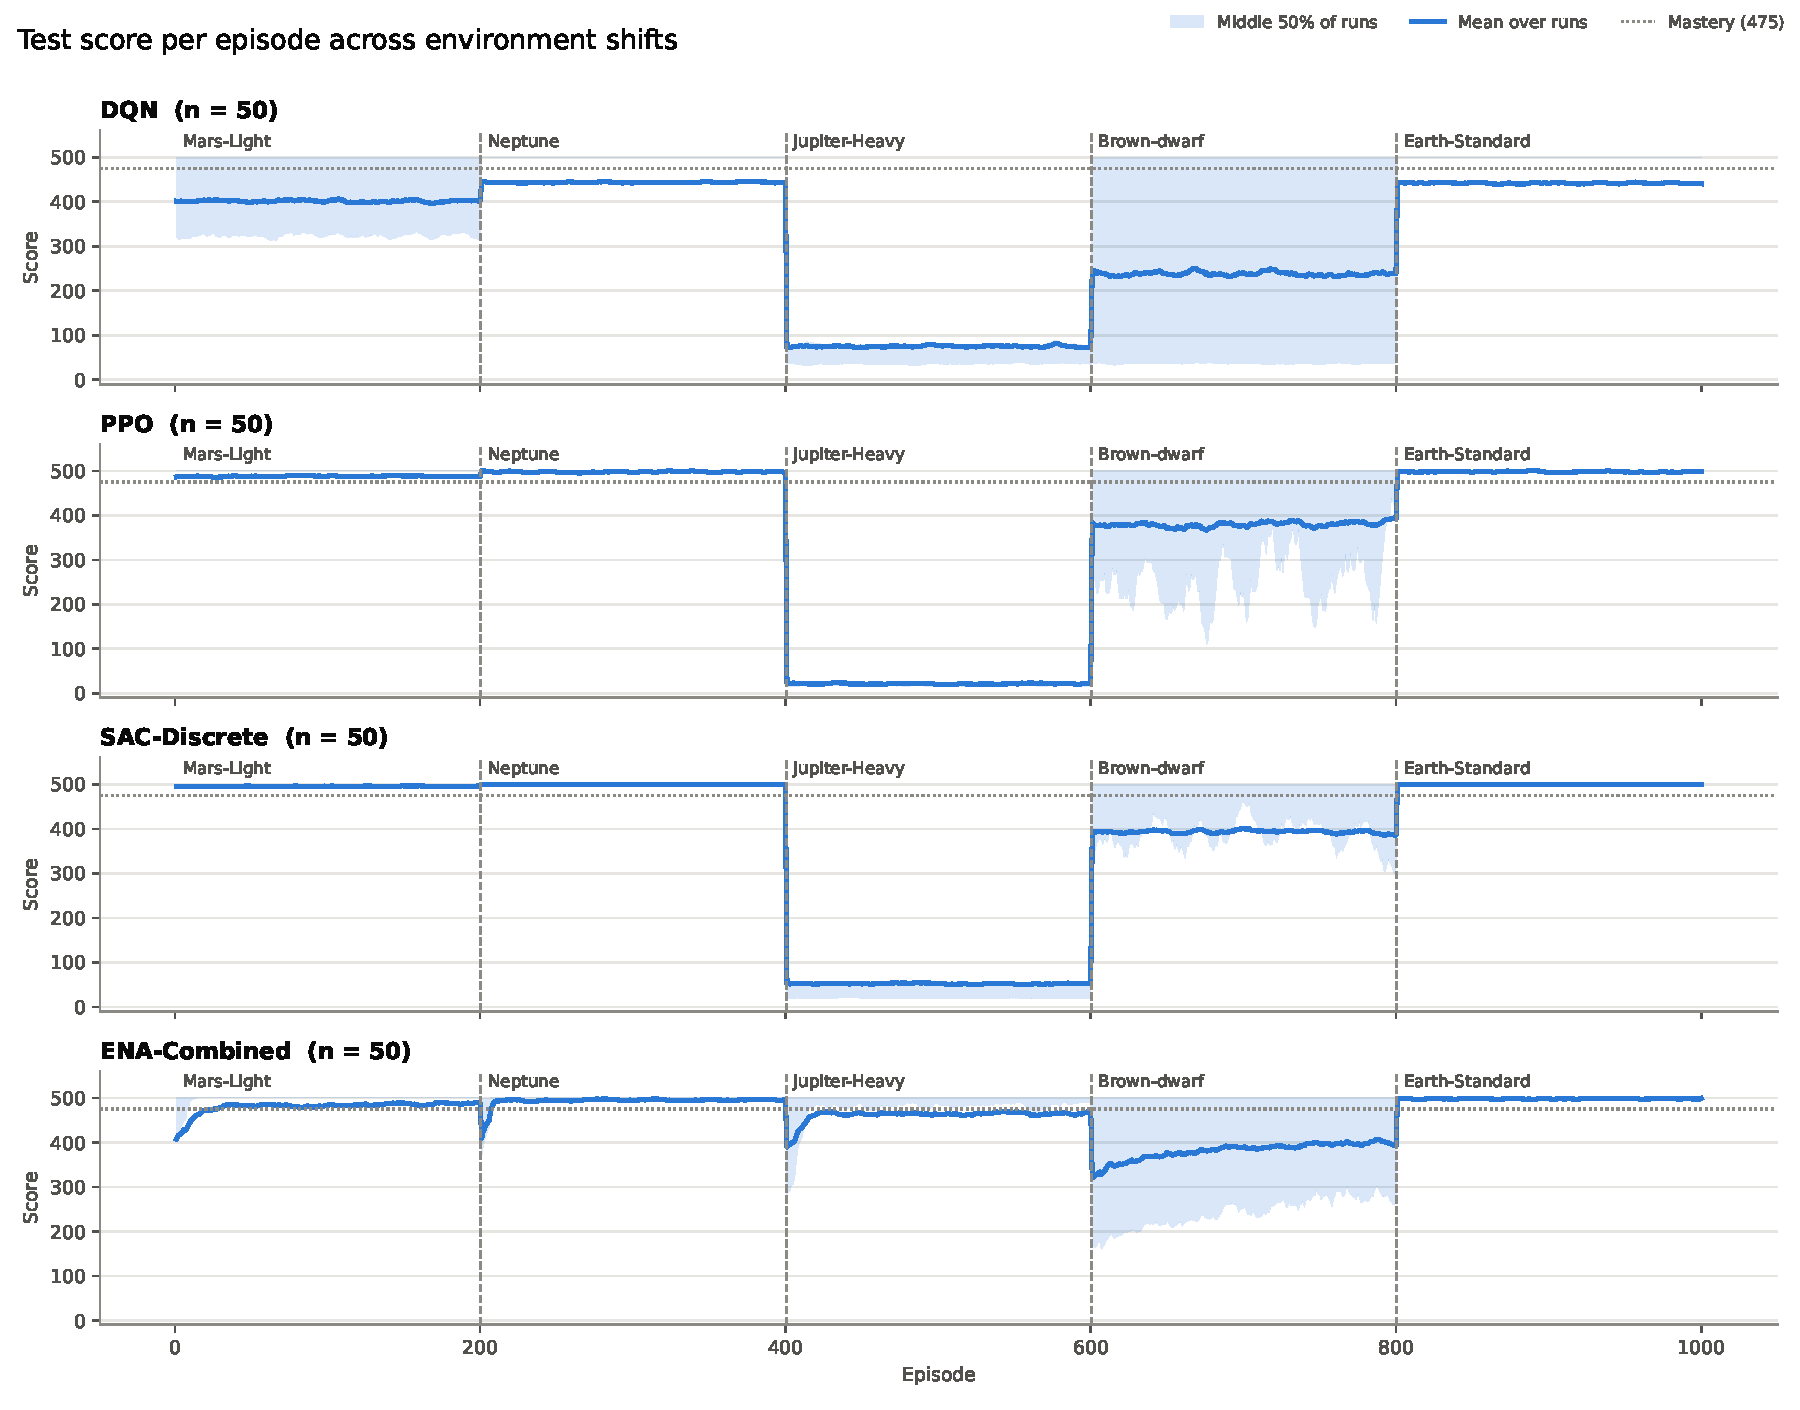
\includegraphics[width=0.85\textwidth]{images/challenge_test_curves.pdf}}
\caption{Frozen test on CartPole: mean return per episode across \Res{challenge/n} replicates (line) and the middle 50\% of replicates (band). Dashed lines mark environment switches; Neptune and Brown-dwarf were never seen in training.}
\label{fig:challenge_curves}
\end{figure*}

\subsection{Frozen Test Dynamics on HalfCheetah}
Fig.~\ref{fig:cheetah_test_curves} illustrates the test phase across the sequential protocol of five environments (50 evaluation episodes per environment): Earth-Standard $\to$ Ice-Floor $\to$ Heavy-Rough $\to$ High-Wind $\to$ Mars-Slippery. Solid lines show the mean test return across all \Res{cheetah/n} replicates, and shaded bands mark the middle 50\% interquartile range.

On \textit{Heavy-Rough} (episodes 101--150), both PPO and SAC suffer catastrophic performance collapse: after having adapted to Mars-Slippery during the final training phase, their frozen policies drop to mean returns of \Res{cheetah/PPO/test/Heavy-Rough/mean} and \Res{cheetah/SAC/test/Heavy-Rough/mean}, respectively. In contrast, ENA-Combined identifies the environment switch via its wavelet-packet chirp and successfully retrieves its archived Heavy-Rough specialist, sustaining a mean return of \Res{cheetah/ENA-Combined/test/Heavy-Rough/mean}.

On the two environments never seen during training (\textit{Ice-Floor} and \textit{High-Wind}), all agents operate zero-shot. SAC's continuous representations achieve high baseline locomotor velocity on Ice-Floor, whereas ENA's chirp identifies these novel physics as unrecognized, falling back on its best-matching archived specialist without catastrophic instability.

\begin{figure*}[t]
\centerline{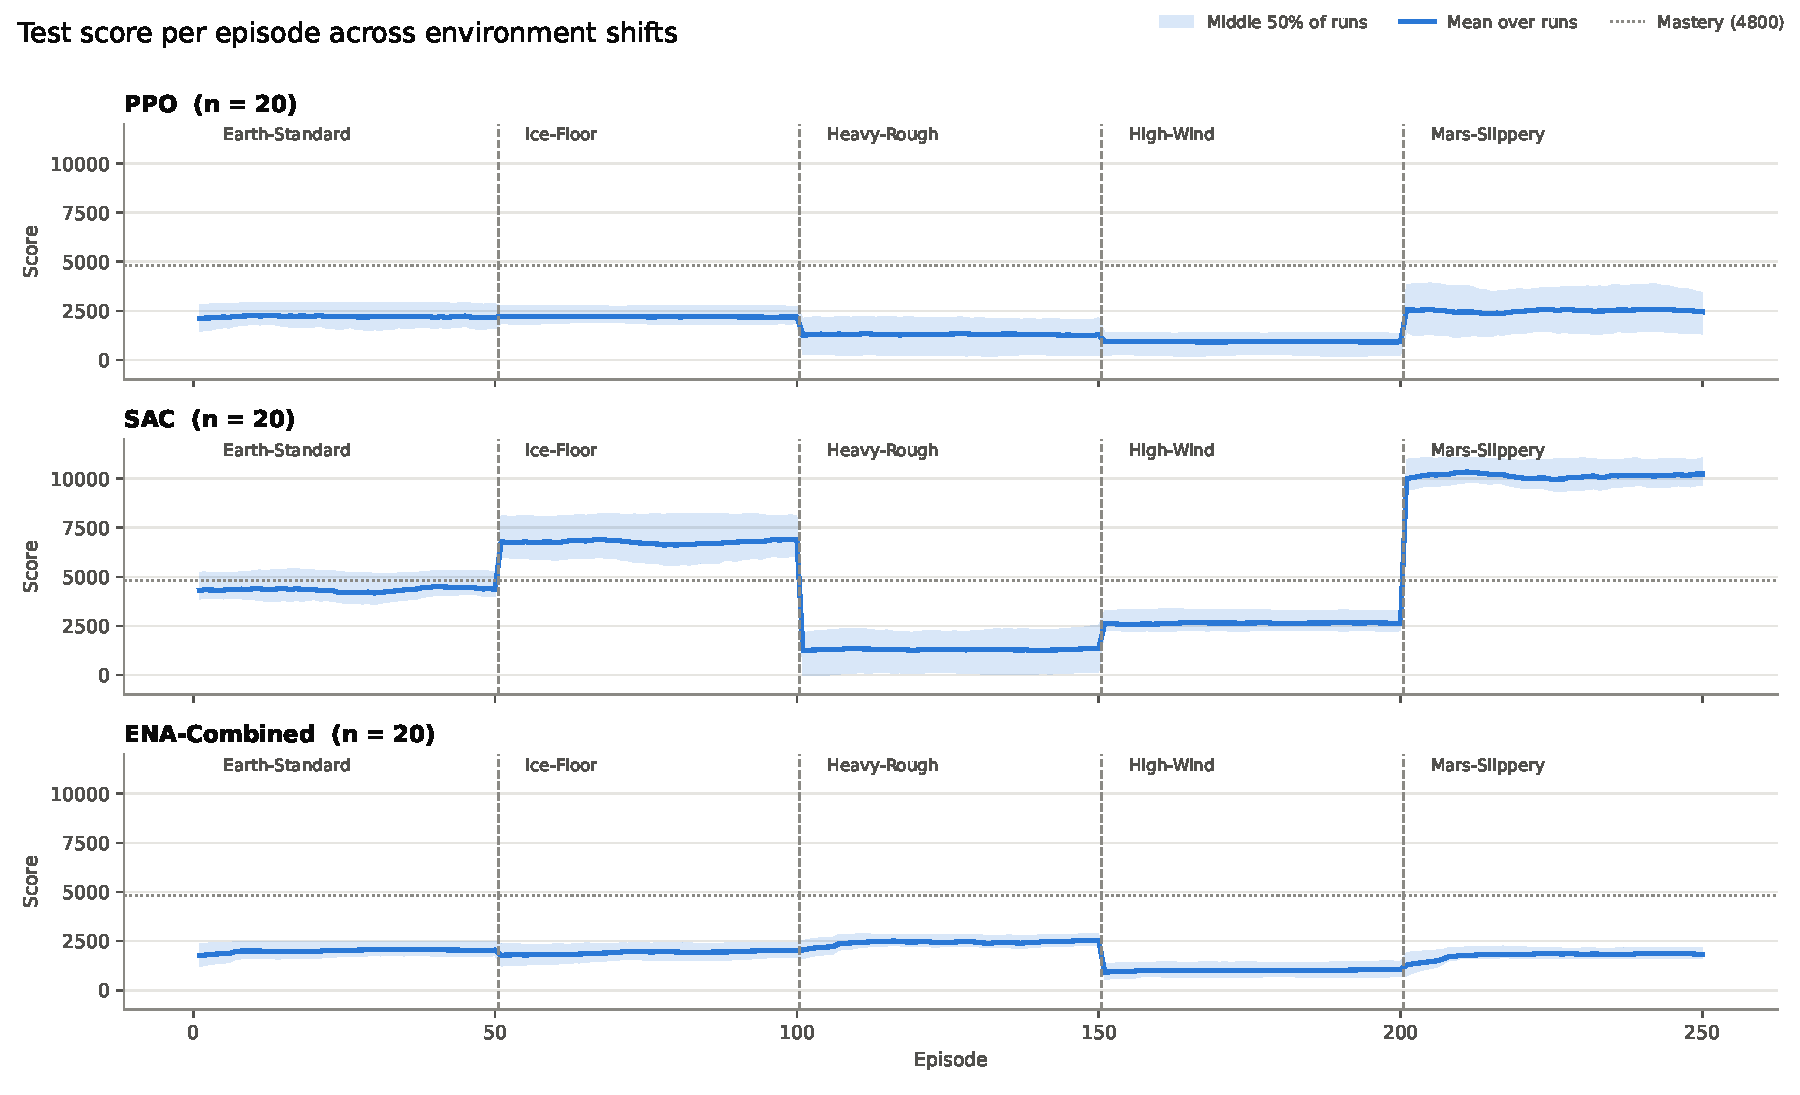
\includegraphics[width=0.85\textwidth]{images/cheetah_test_curves.pdf}}
\caption{Frozen test on HalfCheetah: mean return per episode across \Res{cheetah/n} replicates (line) and middle 50\% interquartile range (band). Dashed vertical lines mark environment transitions; Ice-Floor and High-Wind were never encountered during training. While SAC and PPO suffer severe forgetting on Heavy-Rough, ENA-Combined recalls its archived specialist.}
\label{fig:cheetah_test_curves}
\end{figure*}

\subsection{Training Dynamics Across Sequential Environments}
Fig.~\ref{fig:cheetah_training_curves} displays the training trajectories of all three agents over the full interaction budget of 3,000,000 environment steps (1,000,000 steps per training phase: Earth-Standard $\to$ Heavy-Rough $\to$ Mars-Slippery). Returns are binned and smoothed over step intervals across the \Res{cheetah/n} replicates.

During training, SAC's off-policy gradient optimization rapidly masters each individual environment, climbing to peak returns of $\sim$8,500 on Earth-Standard, $\sim$7,500 on Heavy-Rough, and $\sim$9,500 on Mars-Slippery. However, the sharp discrepancy between SAC's high training return at step $2.0\!\times\!10^6$ on Heavy-Rough and its test return of \Res{cheetah/SAC/test/Heavy-Rough/mean} in Fig.~\ref{fig:cheetah_test_curves} shows how severely this SAC implementation forgets an environment on this sequence once its single policy keeps training on the next one.

ENA-Combined makes steady progress within its interaction budget, achieving end-of-phase training averages of \Res{cheetah/ENA-Combined/end/Earth-Standard/mean} on Earth-Standard and \Res{cheetah/ENA-Combined/end/Heavy-Rough/mean} on Heavy-Rough. Because ENA's step budget is shared between exploratory mutation evaluations, chirp excitation sequences, and active policy execution, its end-of-phase training scores reflect active search variance; when evaluated with frozen elites at test time, it maintains and exceeds these levels (\Res{cheetah/ENA-Combined/test/Earth-Standard/mean} on Earth-Standard, \Res{cheetah/ENA-Combined/test/Heavy-Rough/mean} on Heavy-Rough).

\begin{figure*}[t]
\centerline{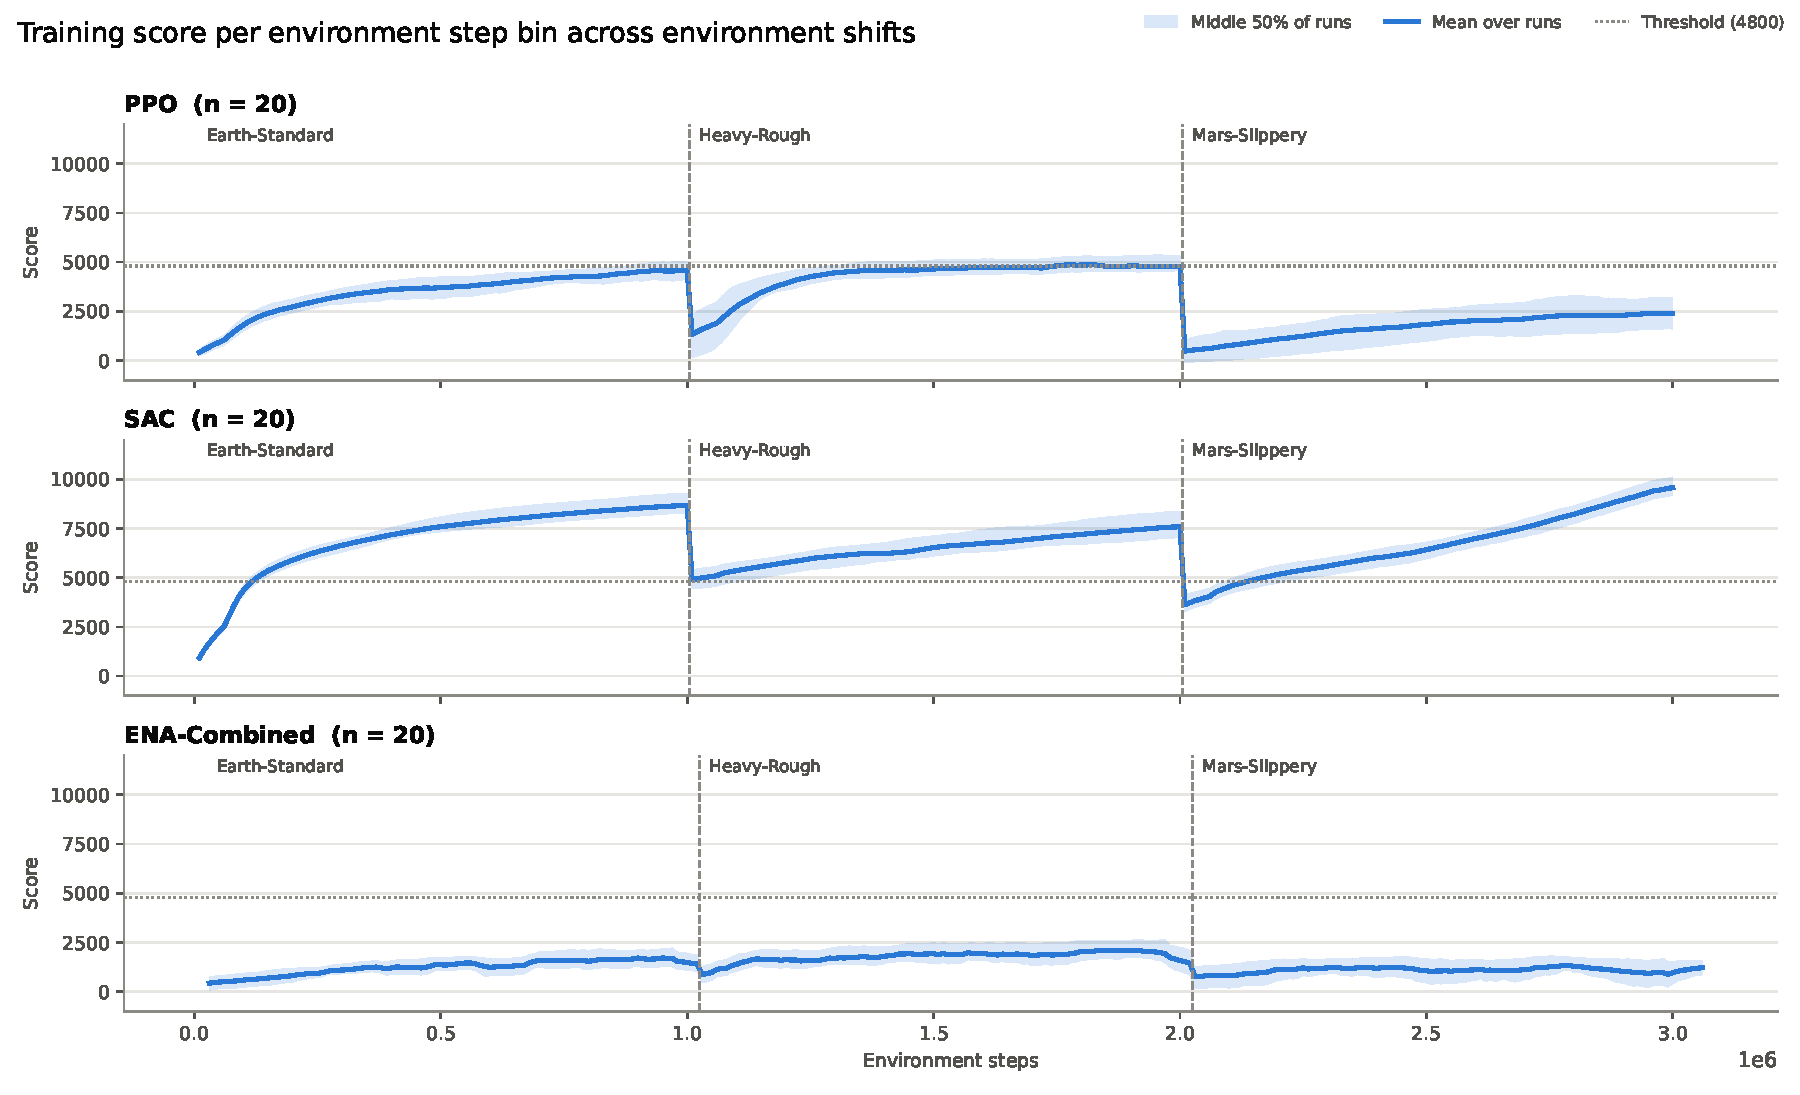
\includegraphics[width=0.85\textwidth]{images/cheetah_training_curves.pdf}}
\caption{Training score binned across environment steps over the 3,000,000-step budget on HalfCheetah (\Res{cheetah/n} replicates; line is mean, band is middle 50\% of replicates). Dashed vertical lines mark transitions between the three sequential training environments (Earth-Standard $\to$ Heavy-Rough $\to$ Mars-Slippery).}
\label{fig:cheetah_training_curves}
\end{figure*}
